% \documentclass[a4paper,10pt]{article}
\documentclass[a4paper,10pt,titlepage]{article}
% \documentclass[a4paper,10pt,twocolumn]{article}
% \documentclass[a4paper,10pt,twocolumn,titlepage]{article}

\usepackage[
	top=1cm,
	bottom=1cm,
	left=2cm,
	right=2cm,
%   twoside,
%   bindingoffset=1cm,
%   asymmetric,
	headheight=0.5cm,
	headsep=0cm,
	footskip=0.5cm,
	includehead=true,
	includefoot=true]{geometry}

\usepackage{./lib/notes}
\usepackage{graphicx}
\usepackage{subfig}
\usepackage{float}
\usepackage{tikz}
\usepackage{xcolor}

% \usepackage{transparent}
% \usepackage{eso-pic}
% \newcommand\BackgroundPic{%
% \put(0,0){%
% \parbox[b][\paperheight]{\paperwidth}{%
% \vfill
% \centering
% {\transparent{0.8} 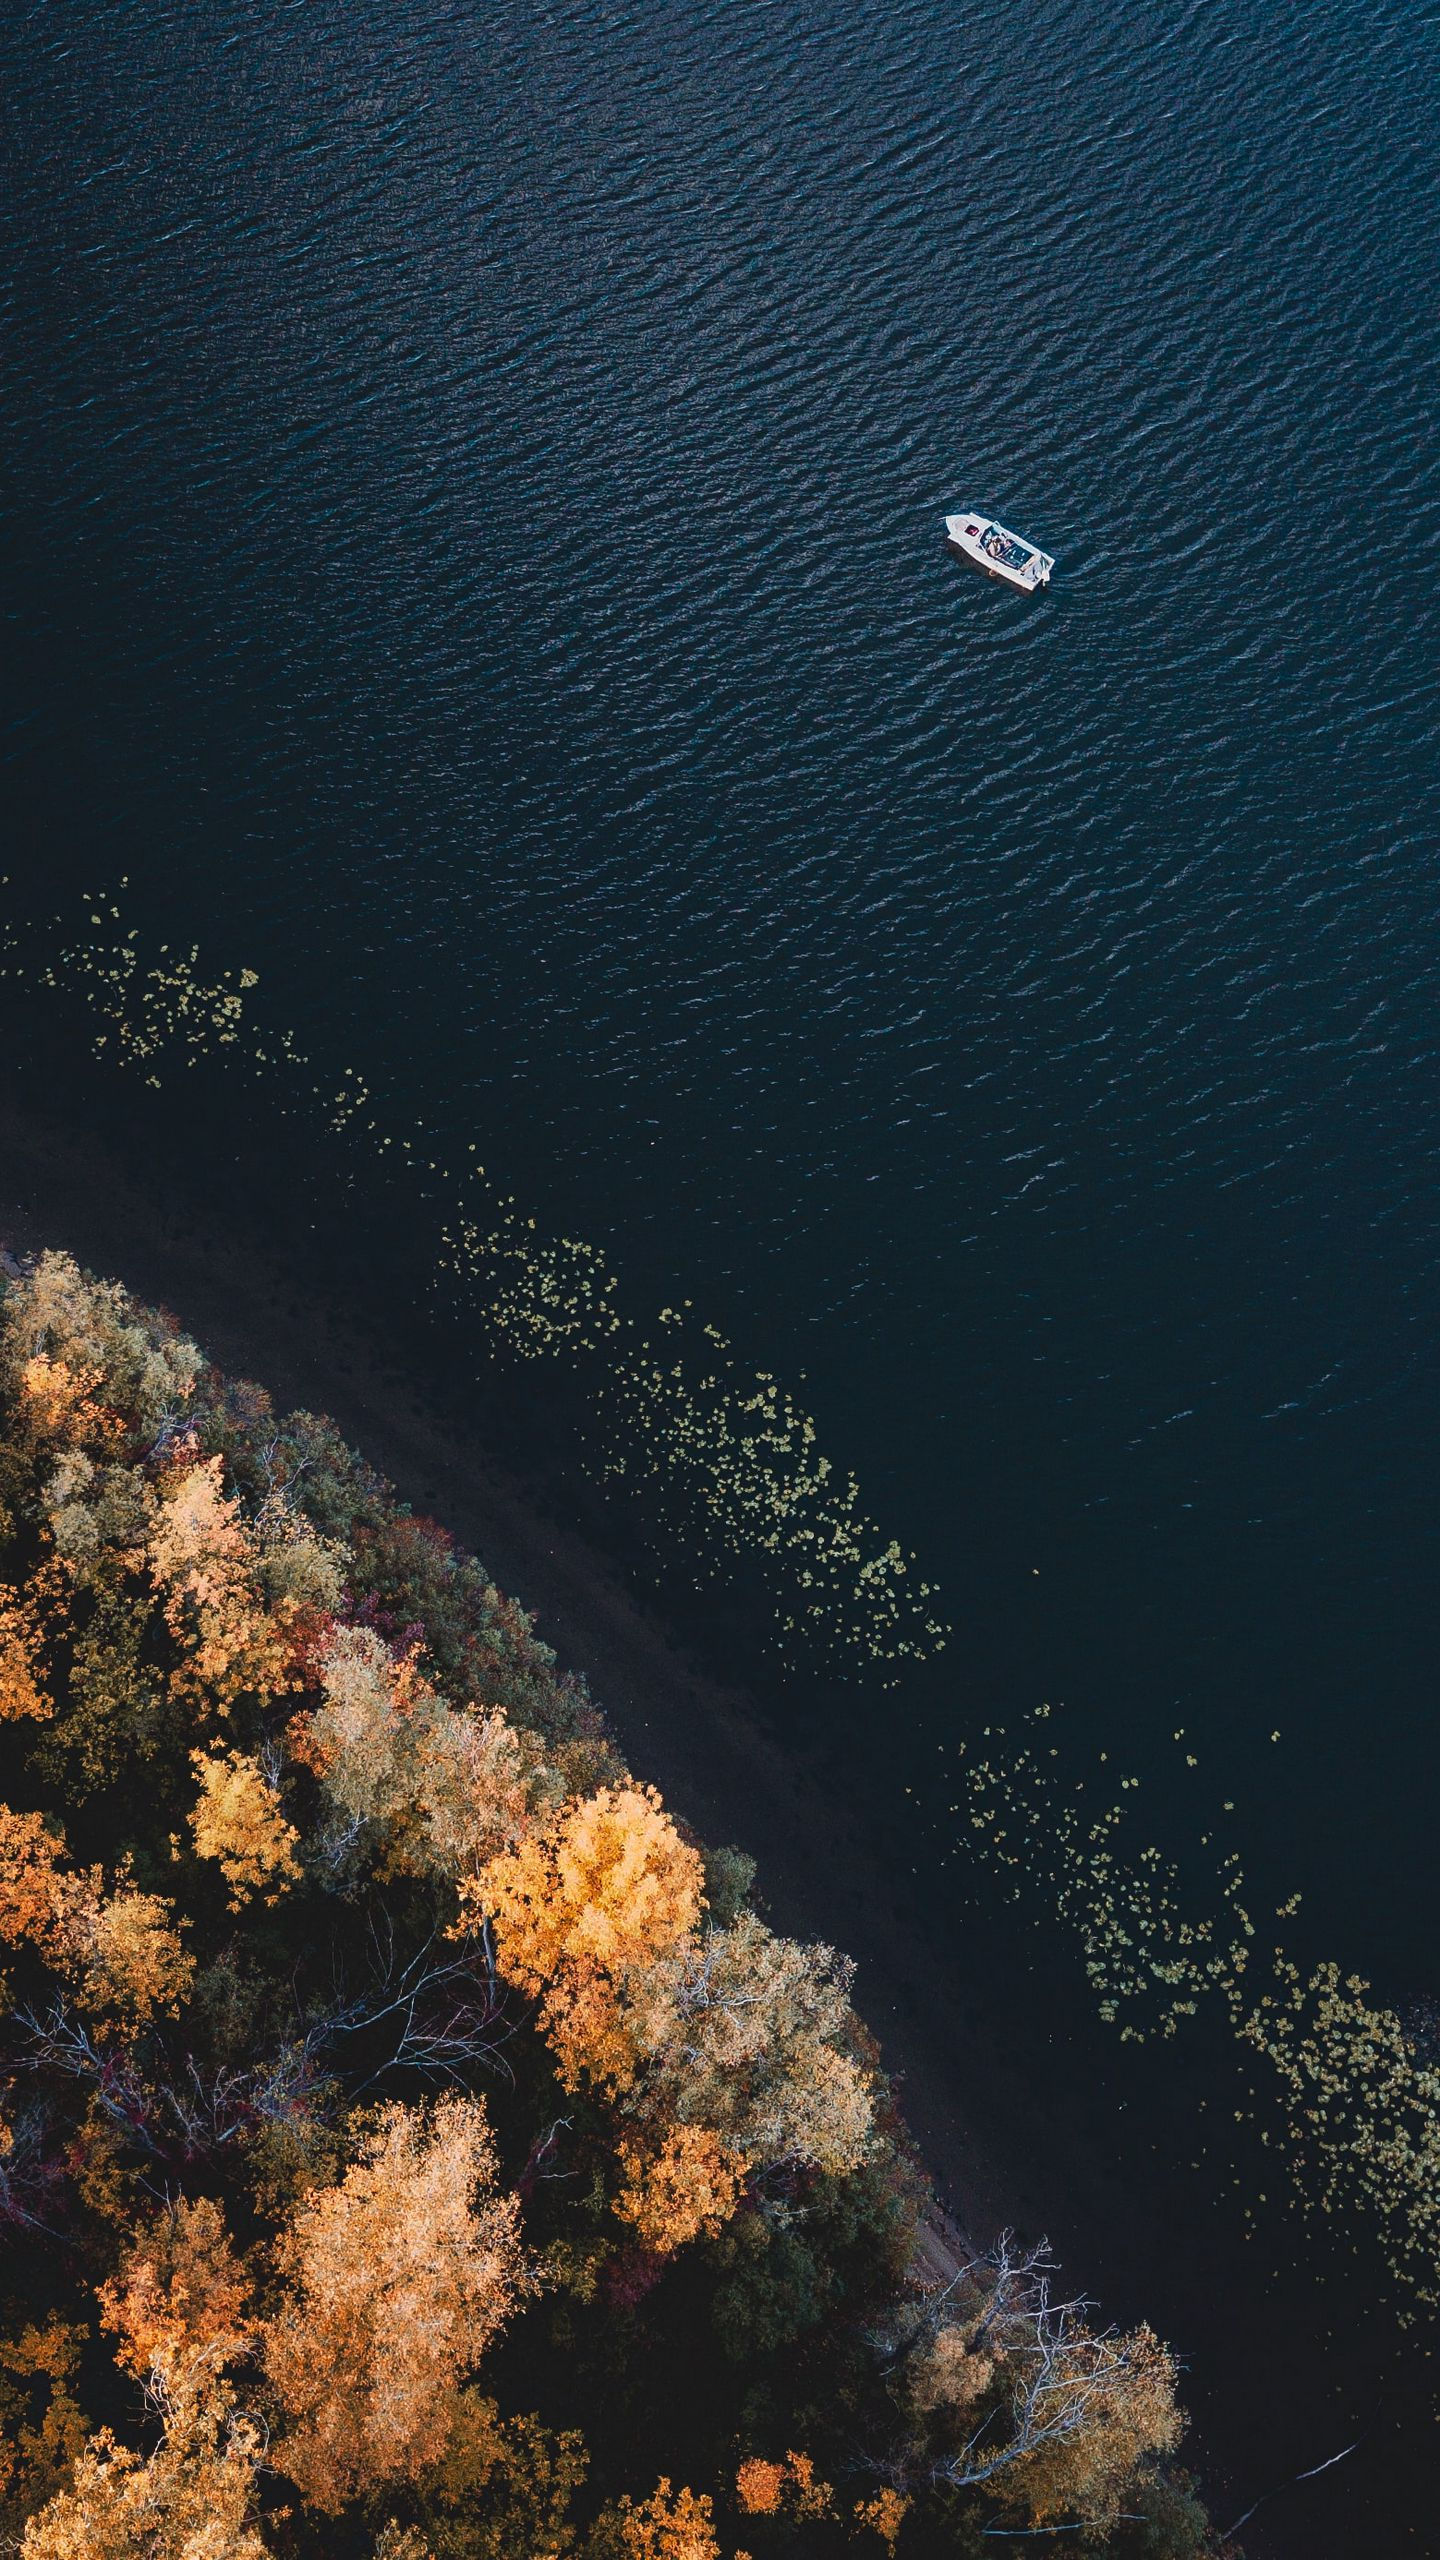
\includegraphics[width=\paperwidth,height=\paperheight,%
% keepaspectratio]{./assets/img/boat_coast_aerial_view_175780_1440x2560.jpg}}%
% \vfill
% }}}

%%%%%%%%%%%%%%%%%%%%%%%%%%%%%%%%%%%%%%%%%%%%%%%%%%%%%%%%%%%%%%%%%%%%%%%%%%%%%%%%
% Basic Info
%%%%%%%%%%%%%%%%%%%%%%%%%%%%%%%%%%%%%%%%%%%%%%%%%%%%%%%%%%%%%%%%%%%%%%%%%%%%%%%%
\title{\Large\bf Formatting Submissions for a USENIX Conference:\\
	An (Incomplete) Example\\
	\hologo{pdfLaTeX}
}
\author{%
    {\rm Ruohong~Jiao}\\
	First Institution
	\and
	{\rm Second~Name}\\
	Second Institution
	\and
	{\rm Third~Name}\\
	Third Institution
	\and
	{\rm Fourth~Name}\\
	Fourth Institution
	\and
	{\rm Fifth~Name}\\
	Fifth Institution
}
\date{2020-03-28}

%%%%%%%%%%%%%%%%%%%%%%%%%%%%%%%%%%%%%%%%%%%%%%%%%%%%%%%%%%%%%%%%%%%%%%%%%%%%%%%%
\begin{document}
%%%%%%%%%%%%%%%%%%%%%%%%%%%%%%%%%%%%%%%%%%%%%%%%%%%%%%%%%%%%%%%%%%%%%%%%%%%%%%%%
% \AddToShipoutPicture*{\BackgroundPic}

\maketitle

%-------------------------------------------------------------------------------
\begin{abstract}
%-------------------------------------------------------------------------------
Your abstract text goes here. Just a few facts. Whet our appetites.
Not more than 200 words, if possible, and preferably closer to 150.
\end{abstract}
%\newpage

%\tableofcontents
%\newpage

%-------------------------------------------------------------------------------
\section{Introduction}
%-------------------------------------------------------------------------------
Some of the \textbf{greatest}\par
discoveries in \underline{science}\par
were made by \textbf{\textit{accident}}.\par

\lipsum[1]

%-------------------------------------------------------------------------------
\section{Footnotes, Verbatim, and Citations}
%-------------------------------------------------------------------------------

Footnotes should be places after punctuation characters, without any
spaces between said characters and footnotes, like so.%
\footnote{Remember that USENIX format stopped using endnotes and is
  now using regular footnotes.} And some embedded literal code may
look as follows.

\begin{verbatim}
int main(int argc, char *argv[]) 
{
    return 0;
}
\end{verbatim}

Now we're going to cite somebody. Watch for the cite tag. Here it
comes. Arpachi-Dusseau and Arpachi-Dusseau co-authored an excellent OS
book, which is also really funny~\cite{arpachiDusseau18:osbook}, and
Waldspurger got into the SIGOPS hall-of-fame due to his seminal paper
about resource management in the ESX hypervisor~\cite{waldspurger02}.

The tilde character (\~{}) in the tex source means a non-breaking
space. This way, your reference will always be attached to the word
that preceded it, instead of going to the next line.

And the `cite' package sorts your citations by their numerical order
of the corresponding references at the end of the paper, ridding you
from the need to notice that, e.g, ``Waldspurger'' appears after
``Arpachi-Dusseau'' when sorting references
alphabetically~\cite{waldspurger02,arpachiDusseau18:osbook}. 

It'd be nice and thoughtful of you to include a suitable link in each
and every bibtex entry that you use in your submission, to allow
reviewers (and other readers) to easily get to the cited work, as is
done in all entries found in the References section of this document.

Now we're going take a look at Section~\ref{sec:figs}, but not before
observing that refs to sections and citations and such are colored and
clickable in the PDF because of the packages we've included.

%-------------------------------------------------------------------------------
\section{Floating Figures and Lists}
\label{sec:figs}
%-------------------------------------------------------------------------------


%---------------------------
\begin{figure}
\begin{center}
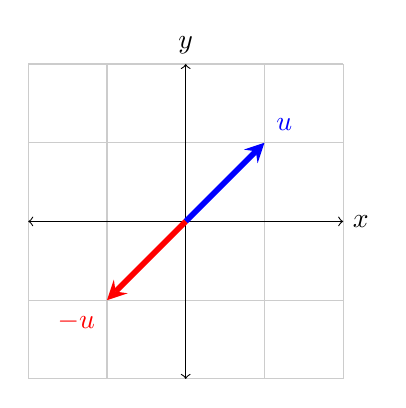
\begin{tikzpicture}
  \draw[thin,gray!40] (-2,-2) grid (2,2);
  \draw[<->] (-2,0)--(2,0) node[right]{$x$};
  \draw[<->] (0,-2)--(0,2) node[above]{$y$};
  \draw[line width=2pt,blue,-stealth](0,0)--(1,1)
        node[anchor=south west]{$\boldsymbol{u}$};
  \draw[line width=2pt,red,-stealth](0,0)--(-1,-1)
        node[anchor=north east]{$\boldsymbol{-u}$};
\end{tikzpicture}
\end{center}
\caption{\label{fig:vectors} Text size inside figure should be as big as
  caption's text. Text size inside figure should be as big as
  caption's text. Text size inside figure should be as big as
  caption's text. Text size inside figure should be as big as
  caption's text. Text size inside figure should be as big as
  caption's text. }
\end{figure}
%% %---------------------------

\begin{figure}[!htbp]
	\centering
	\subfloat[GMM init]{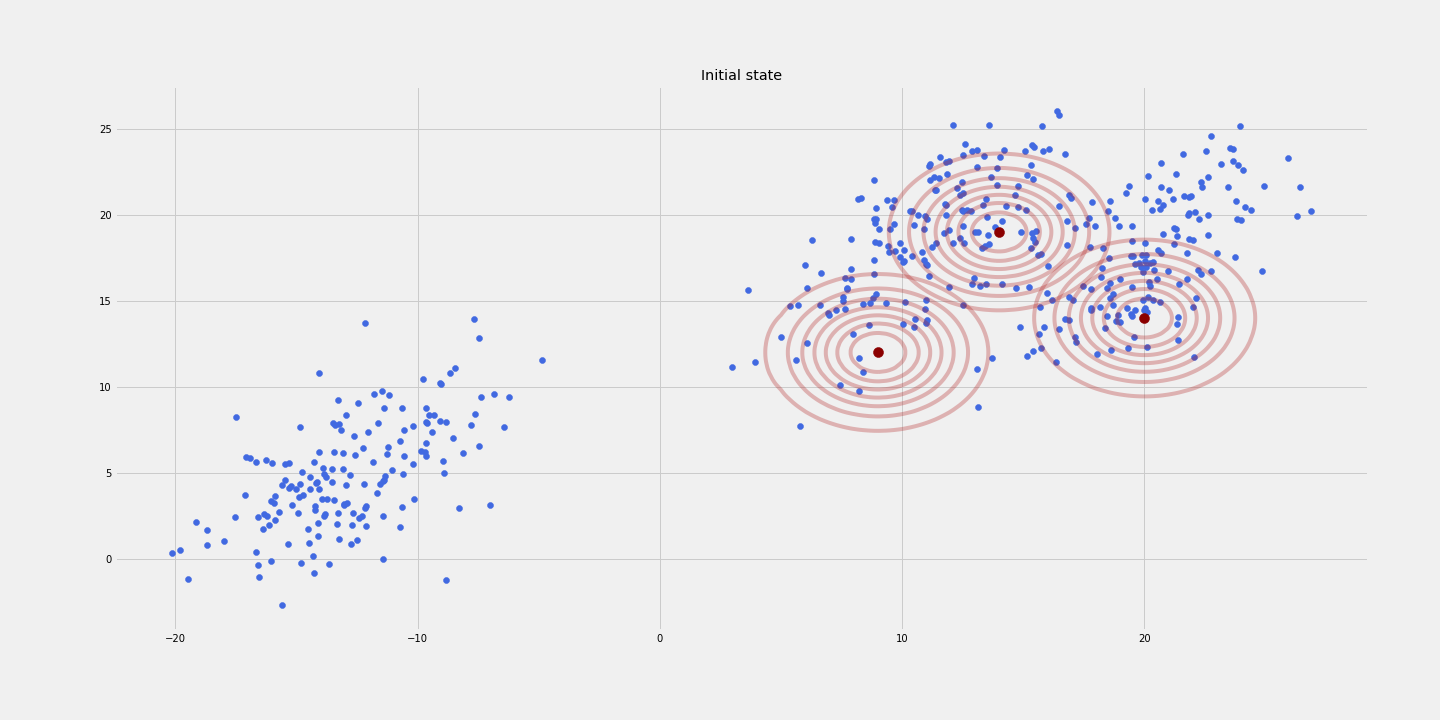
\includegraphics[width=0.4\linewidth]{./assets/img/gmm_init.png}}
	\subfloat[GMM likehood]{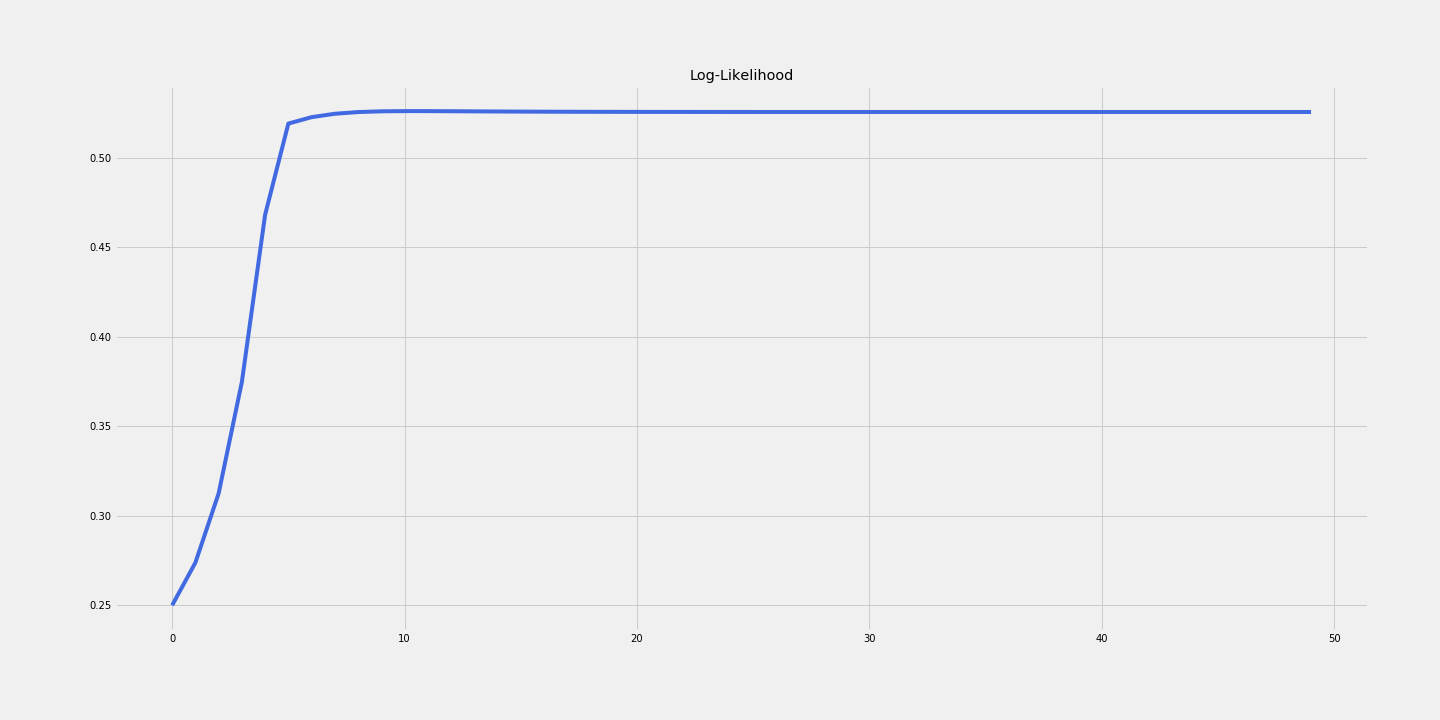
\includegraphics[width=0.4\linewidth]{./assets/img/gmm_like.png}}\\
	\subfloat[GMM ans]{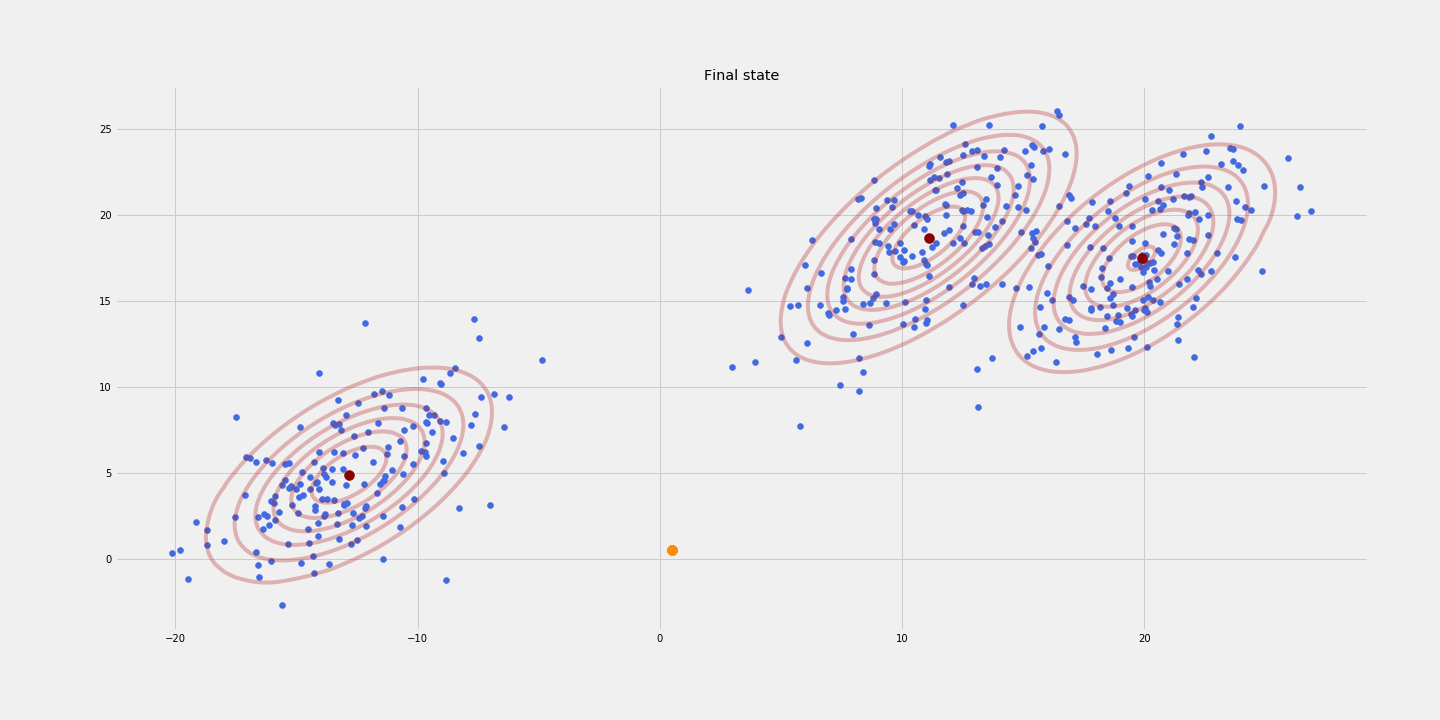
\includegraphics[width=0.8\linewidth]{./assets/img/gmm_ans.png}}
	\caption{GMM}
	\label{fig:gmm}
\end{figure}

Here's a typical reference to a floating figure:
Figure~\ref{fig:vectors}. Floats should usually be placed where latex
wants then. Figure\ref{fig:vectors} is centered, and has a caption
that instructs you to make sure that the size of the text within the
figures that you use is as big as (or bigger than) the size of the
text in the caption of the figures. Please do. Really.

In our case, we've explicitly drawn the figure inlined in latex, to
allow this tex file to cleanly compile. But usually, your figures will
reside in some file.pdf, and you'd include them in your document
with, say, \textbackslash{}includegraphics.

Lists are sometimes quite handy. If you want to itemize things, feel
free:

\begin{description}
  
\item[fread] a function that reads from a \texttt{stream} into the
  array \texttt{ptr} at most \texttt{nobj} objects of size
  \texttt{size}, returning returns the number of objects read.

\item[Fred] a person's name, e.g., there once was a dude named Fred
  who separated usenix.sty from this file to allow for easy
  inclusion.
\end{description}

\noindent
The noindent at the start of this paragraph in its tex version makes
it clear that it's a continuation of the preceding paragraph, as
opposed to a new paragraph in its own right.


\subsection{LaTeX-ing Your TeX File}
%-----------------------------------

People often use \texttt{pdflatex} these days for creating pdf-s from
tex files via the shell. And \texttt{bibtex}, of course. Works for us.

%-------------------------------------------------------------------------------
\section*{Acknowledgments}
%-------------------------------------------------------------------------------

The USENIX latex style is old and very tired, which is why
there's no \textbackslash{}acks command for you to use when
acknowledging. Sorry.

%-------------------------------------------------------------------------------
\section*{Availability}
%-------------------------------------------------------------------------------

USENIX program committees give extra points to submissions that are
backed by artifacts that are publicly available. If you made your code
or data available, it's worth mentioning this fact in a dedicated
section.

%-------------------------------------------------------------------------------
\bibliographystyle{plain}
\bibliography{./bib/reference}

%-------------------------------------------------------------------------------
\begin{appendices}
\section{Some Codes}
some text
\section{Codes}
\lstinputlisting[language=Python]{./assets/files/week5.py}
\end{appendices}

%%%%%%%%%%%%%%%%%%%%%%%%%%%%%%%%%%%%%%%%%%%%%%%%%%%%%%%%%%%%%%%%%%%%%%%%%%%%%%%%
\end{document}
%%%%%%%%%%%%%%%%%%%%%%%%%%%%%%%%%%%%%%%%%%%%%%%%%%%%%%%%%%%%%%%%%%%%%%%%%%%%%%%%

